\chapter{Hero Run Data Analysis} 
\label{chapter5}

Talk about the fully scaled version of Early Earth: the HiPerGator \textit{hero run}

\section{Molfind}
\label{sec:molfind}

\subsection{GraphMatcher}
\label{subsec:molfind_graphmatcher}

\begin{flushleft}
\begin{multiFigure}
    \addFigure{0.5}{Images/early_earth/remakenot_alanine.png}
    \addFigure{0.5}{Images/early_earth/remakenot_alanine_silhouette.png}
\captionof{figure}[Mismatched structure of alanine]{
(A) Structure identified as alanine; 
(B) how the GraphMatcher was interpreting this structure, which makes it appear to be an alanine molecule.}
\label{fig:mismatched_alanine}
\end{multiFigure}
\end{flushleft}

\begin{figure}[!ht]
    \centering
    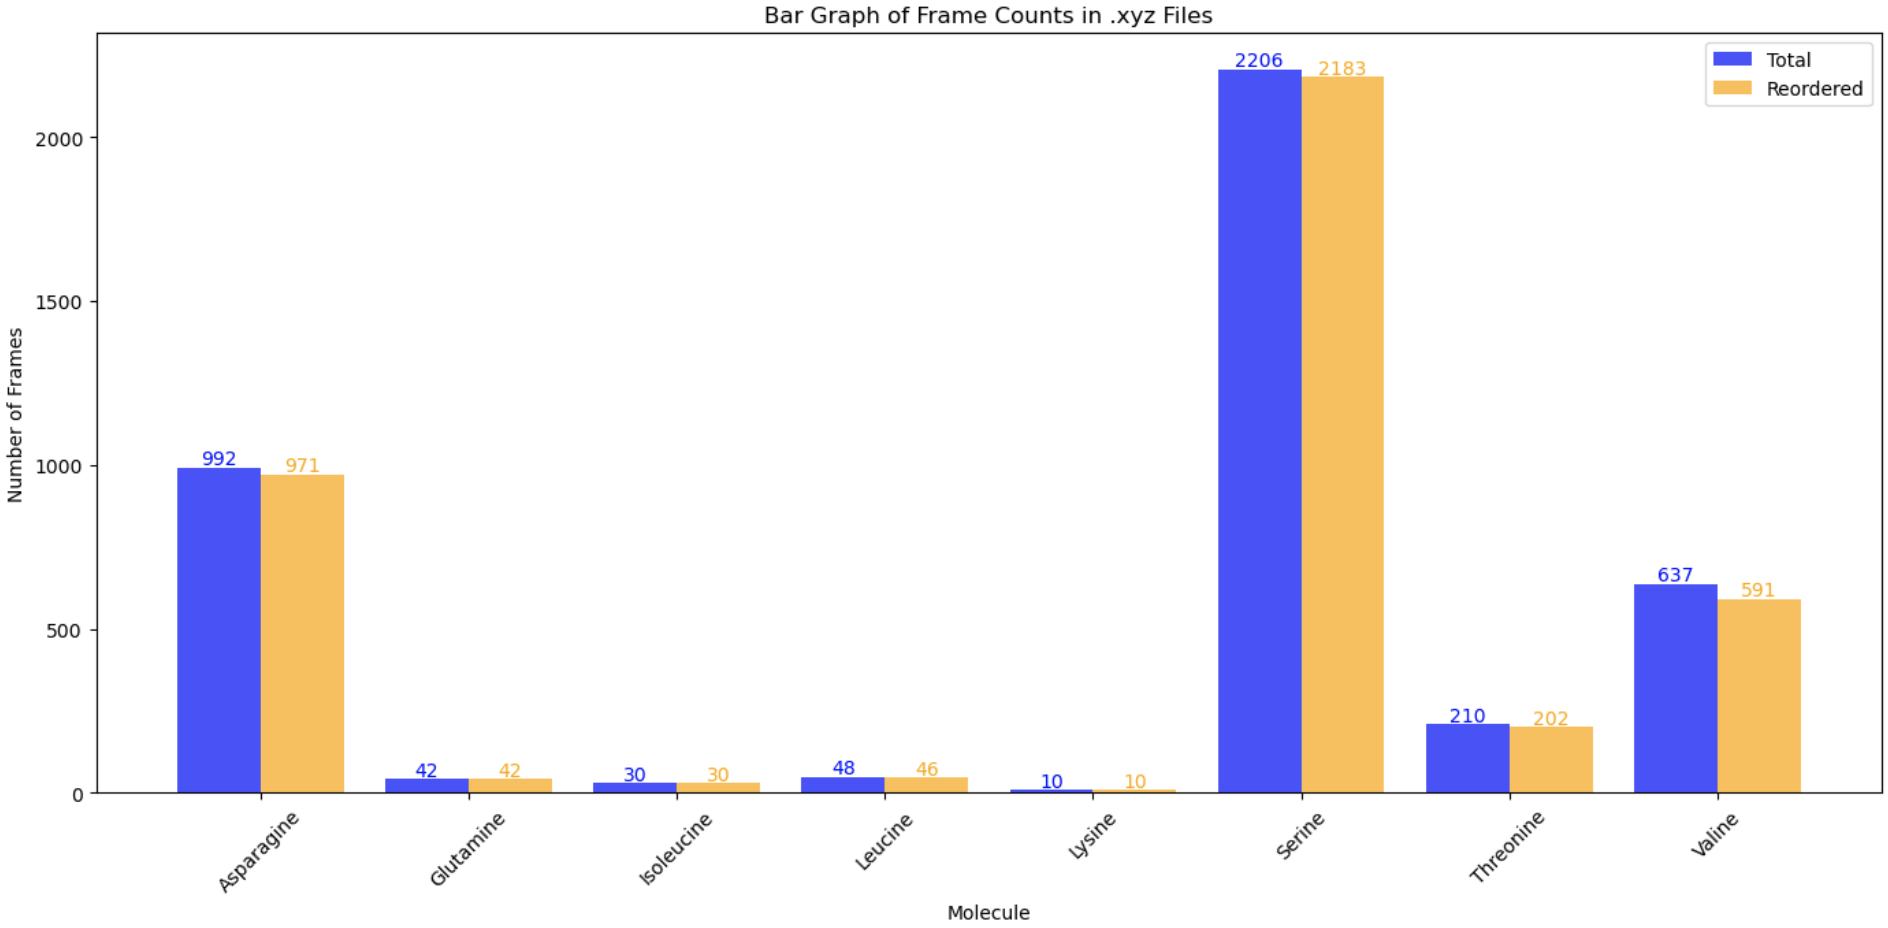
\includegraphics[width=1\linewidth]{Images/early_earth/remake_graph_matching.png}
    \caption[Molecules identified incorrectly in the initial search]{Molecule counts (excluding glycine and alanine) before and after correcting the graph-matching algorithm to account for the proper configuration.}
    \label{fig:graph_matching}
\end{figure}{}

\begin{figure}[!ht]
    \centering
    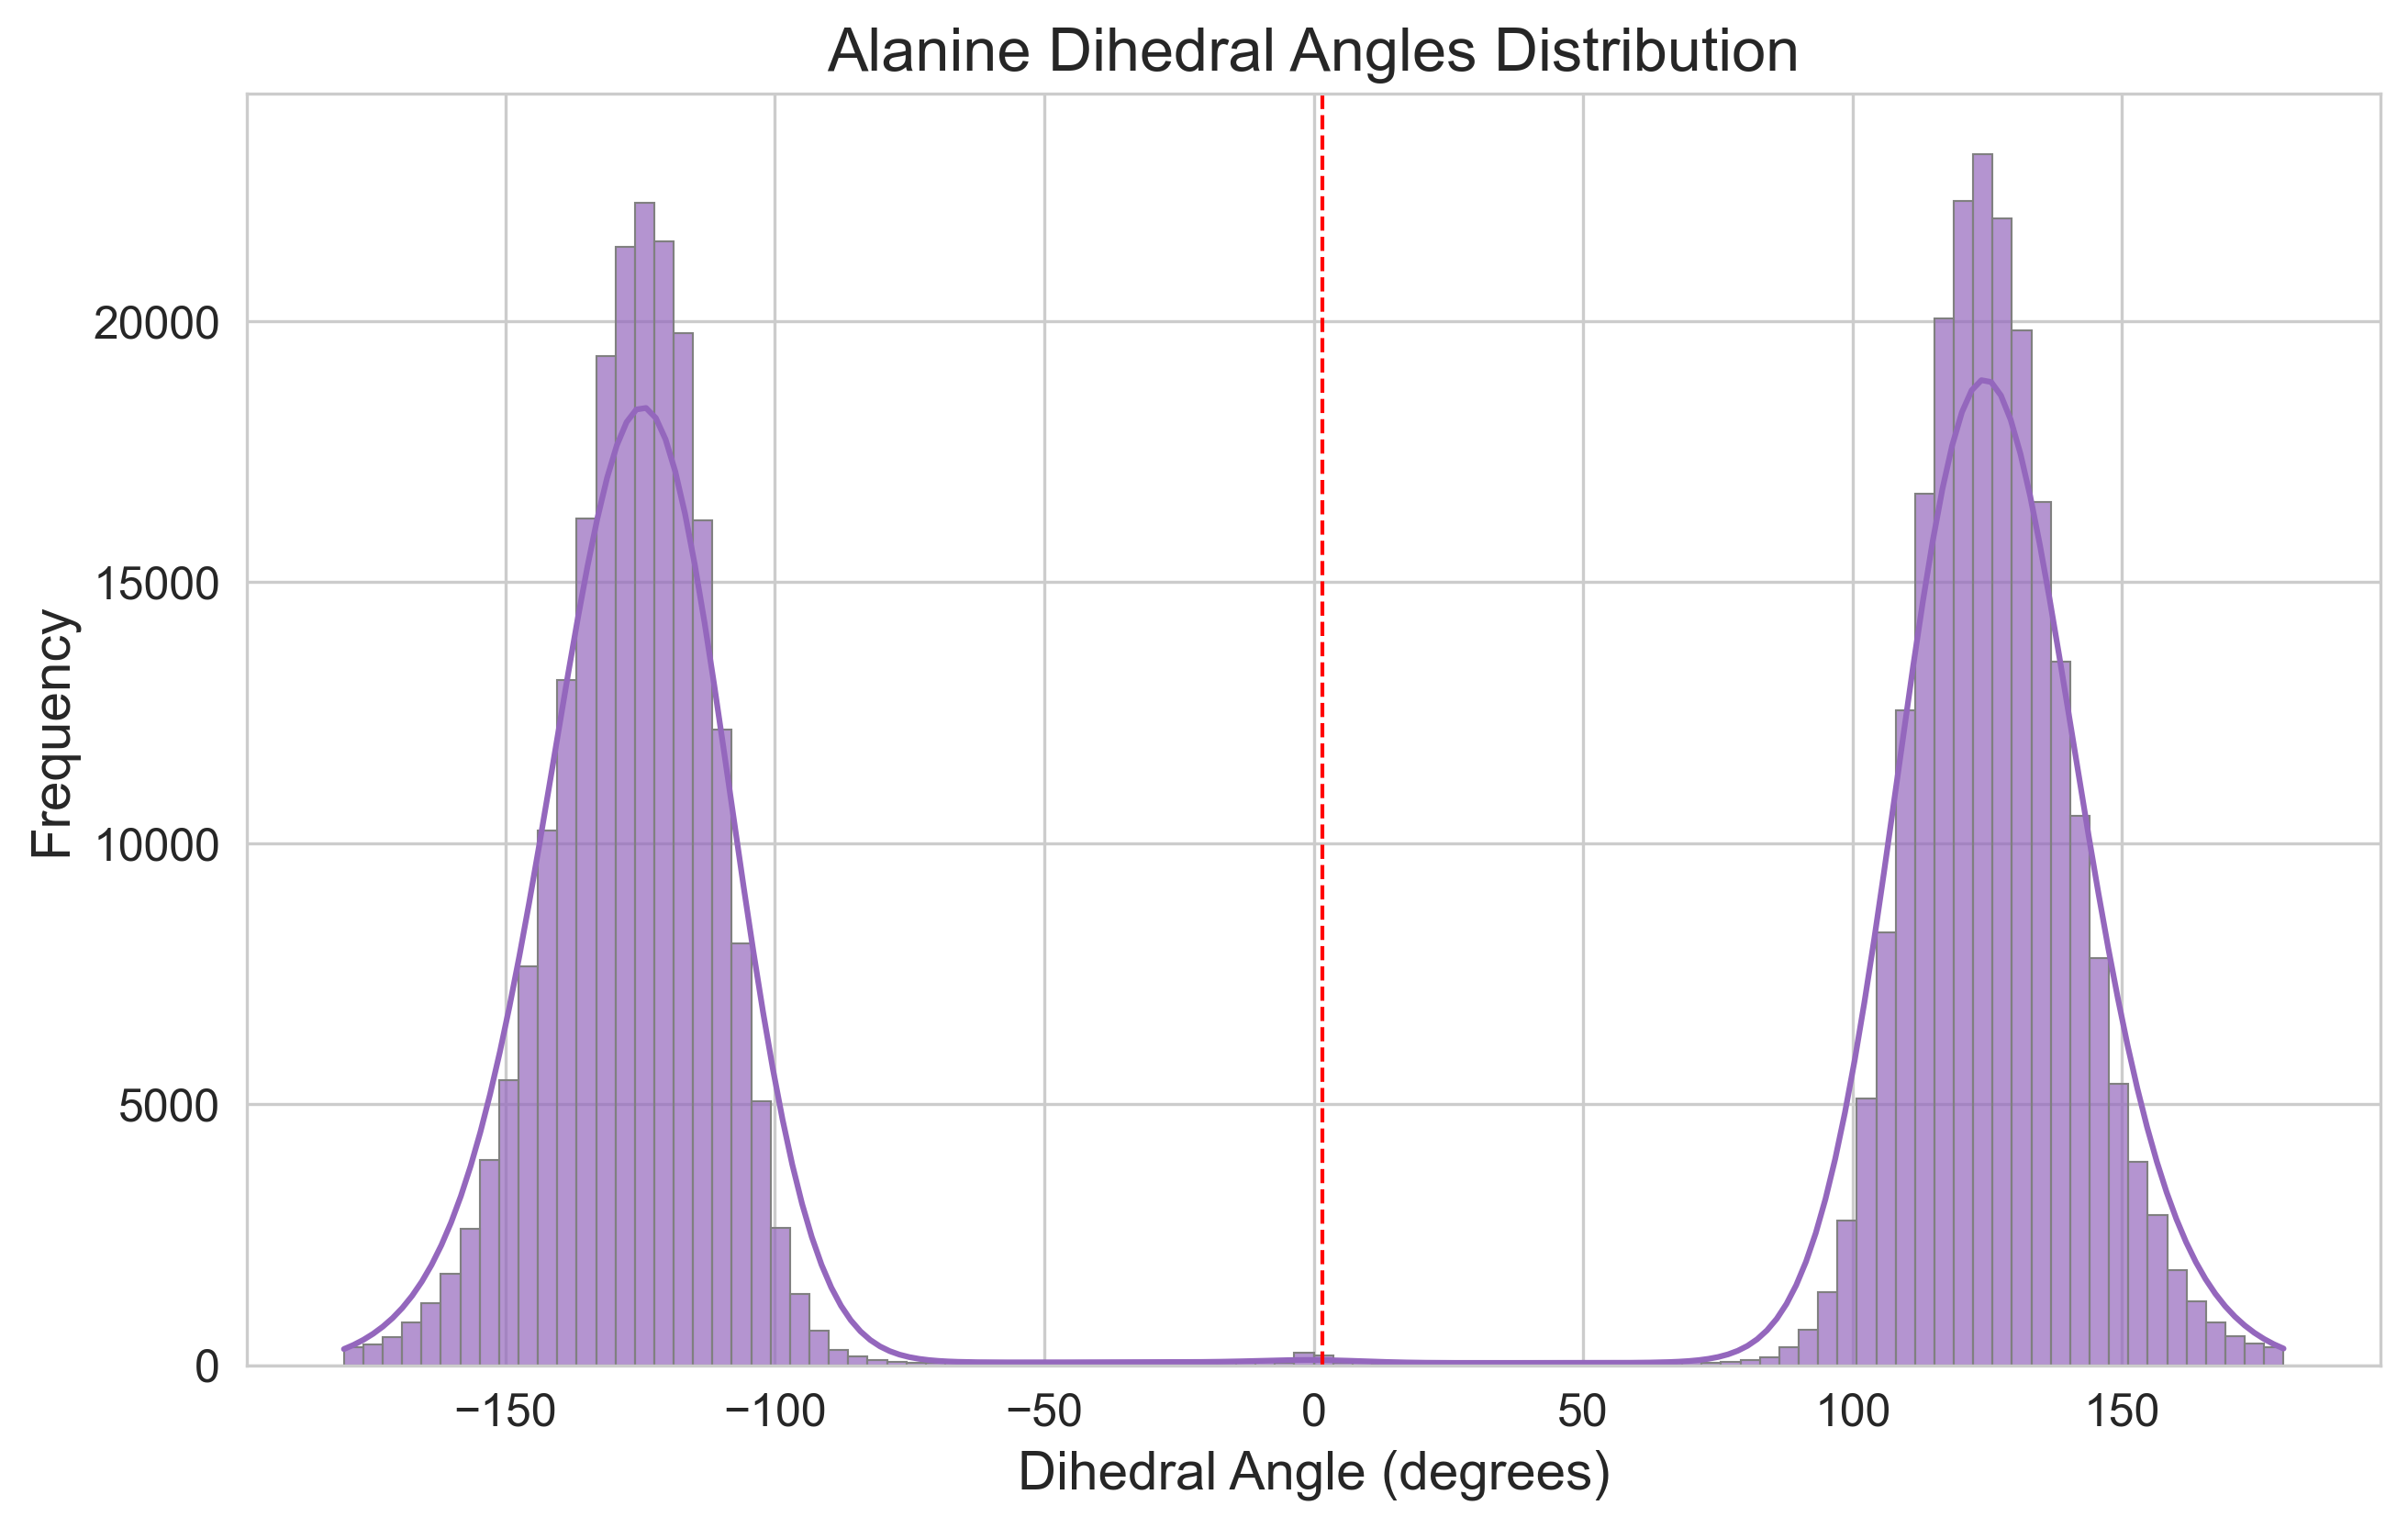
\includegraphics[width=1\linewidth]{Images/alanine_dihedral/dihedral_angles_distribution.png}
    \caption[Distribution of synthesized alanine dihedral angles]{Distribution of dihedral angles in alanine molecules synthesized in the early earth simulation run. Structures obtained from the initial graph search, post-processed with refined graph matching. All molecules fall within the expected range of dihedral angles, centered at $\pm$125$^\circ$.}
    \label{fig:ala_dihedral}
\end{figure}{}

\subsection{Parallelization}
\label{subsec:molfind_parallelization}

\section{Restarts -- Quench analysis}
\label{sec:restarts_quench_analysis}

\begin{figure}[!hp]
    \centering
    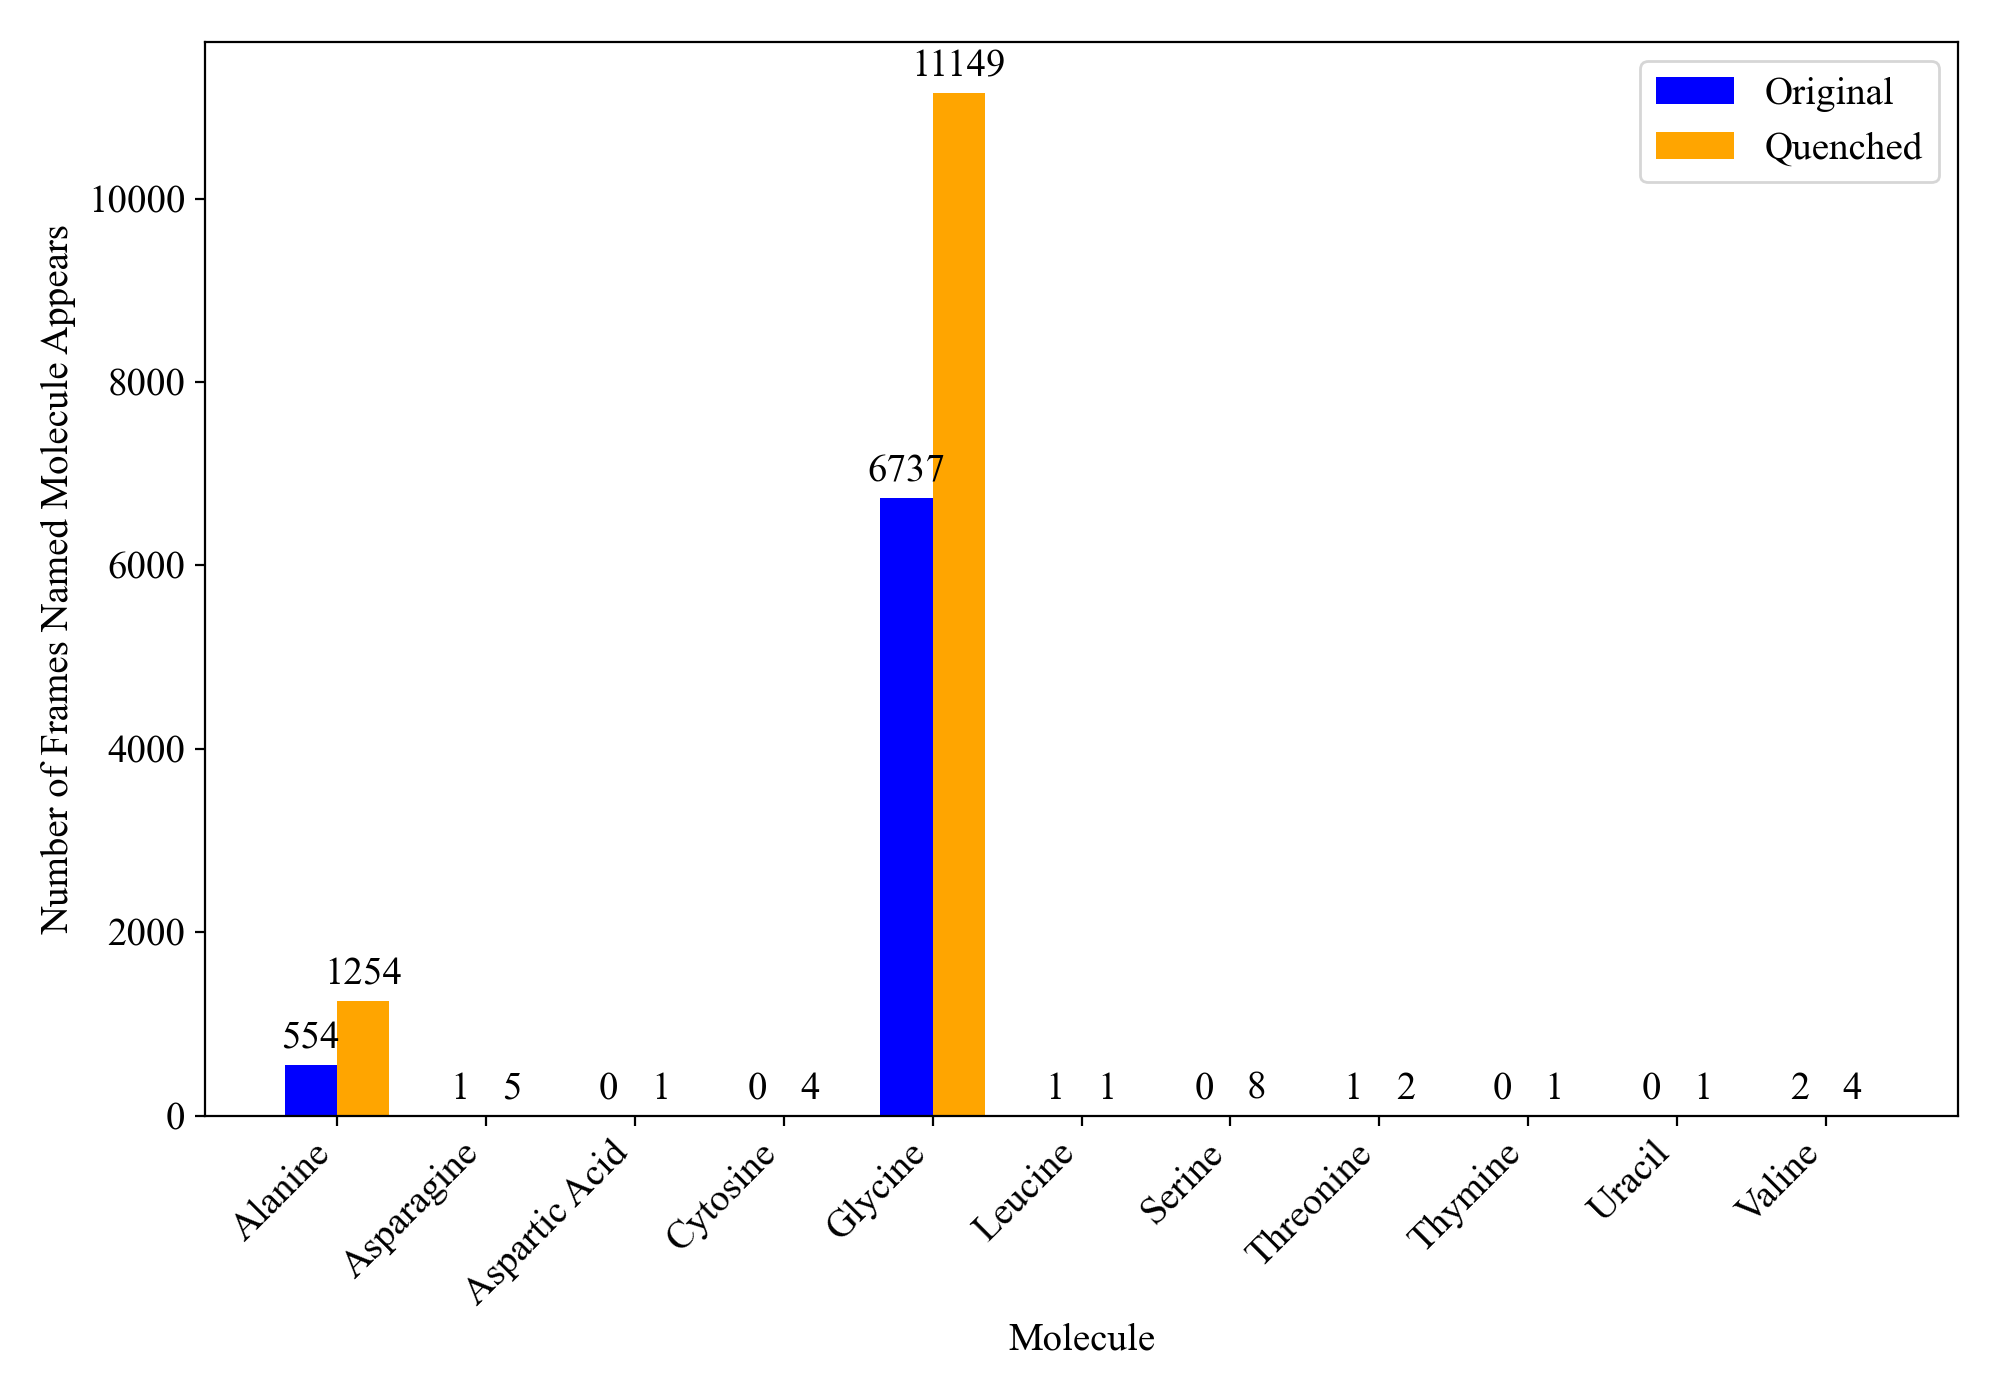
\includegraphics[width=1\linewidth]{Images/early_earth/hist-before-after-quench.png}
    \caption[Histogram: molecules found before and after quenching large early earth system]{Histogram of named molecules found before and after quenching 415 selected frames from the 22.8M atom system from 2500 K to 300 K.}
    \label{fig:ee_quench_hist}
\end{figure}

\begin{figure}[!hp]
    \centering
    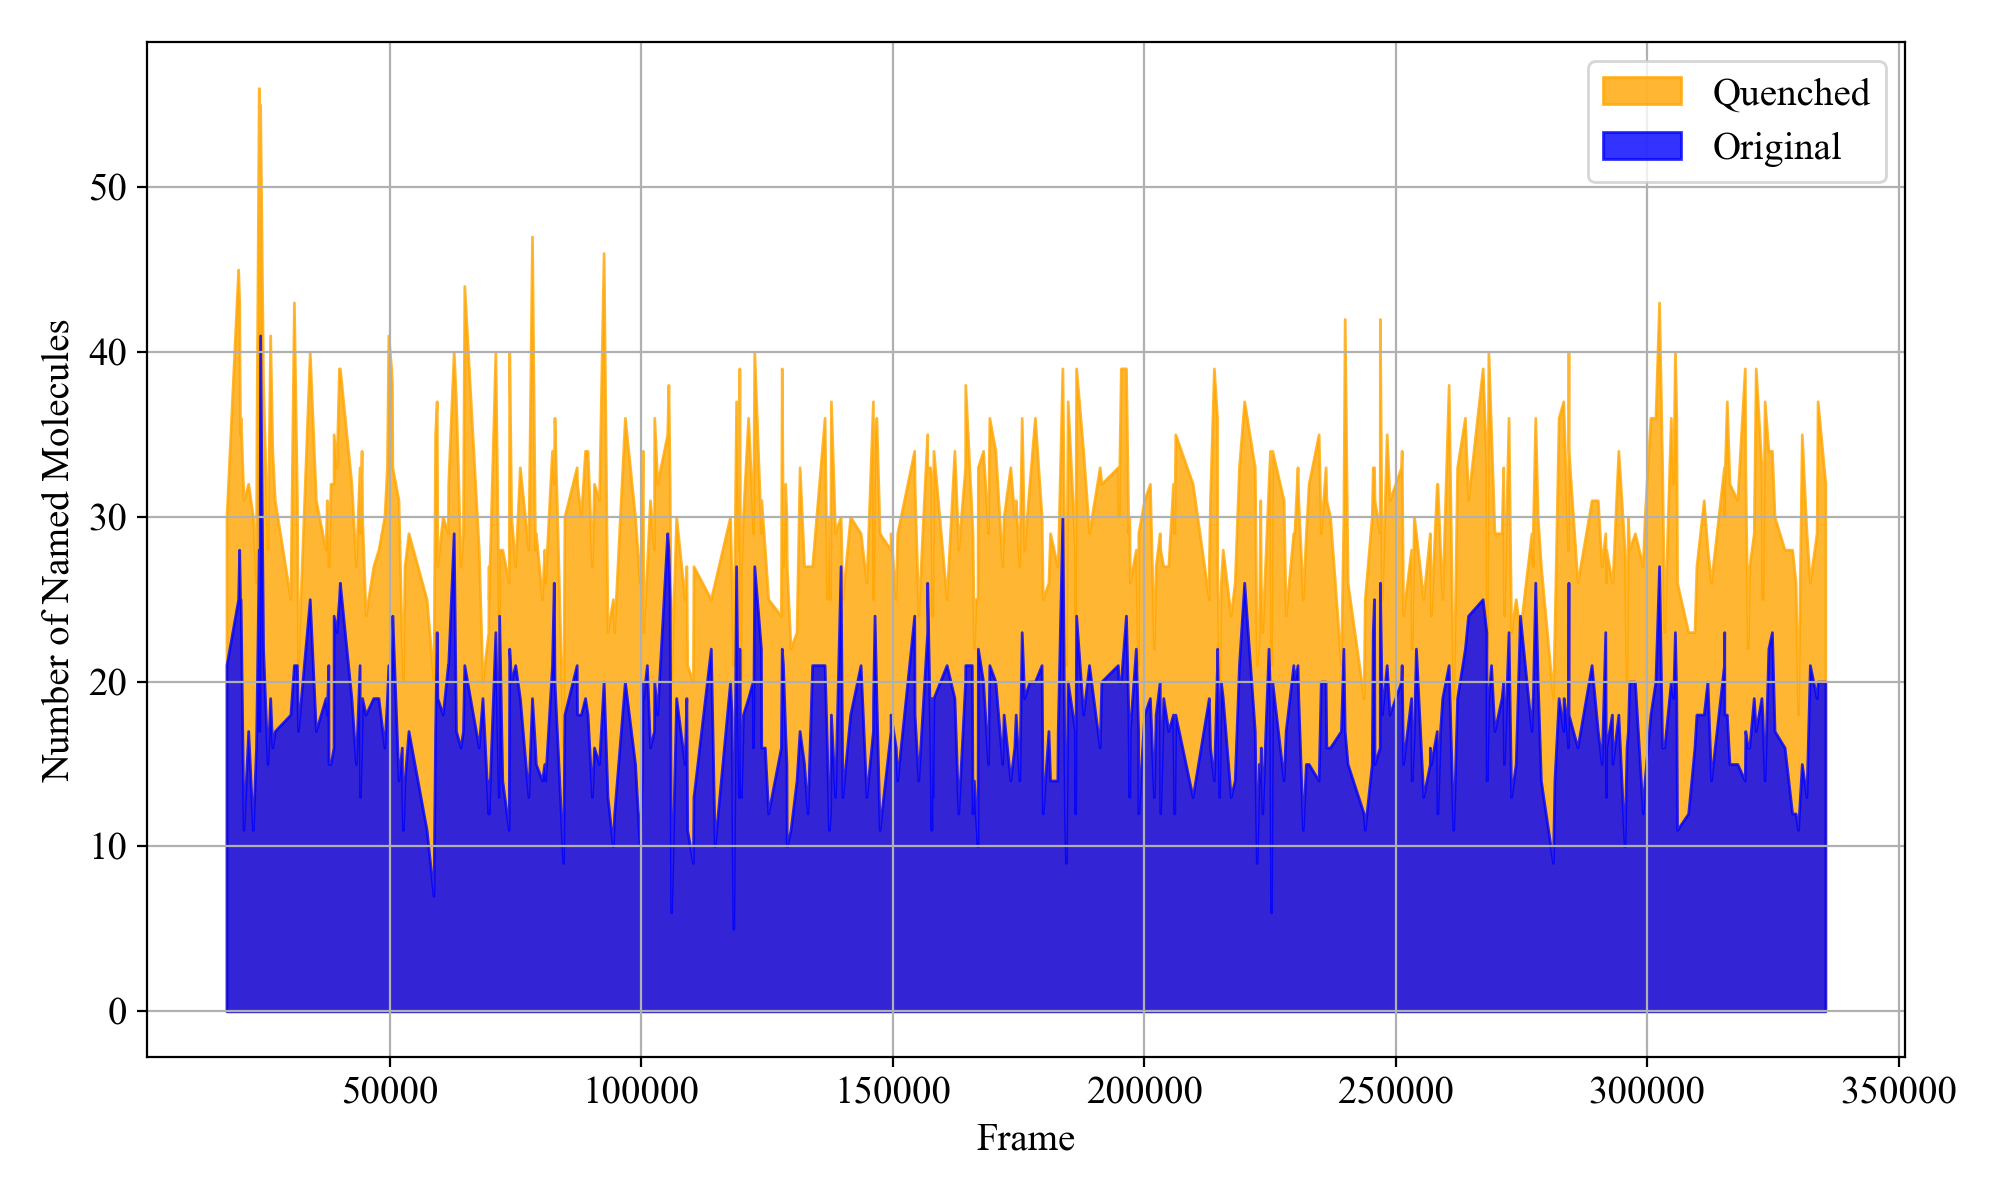
\includegraphics[width=1\linewidth]{Images/early_earth/mol_counts-before-after-quench.png}
    \caption[Line plot: total named molecules found before and after quenching large early earth system]{Total per-frame count of named molecules found before and after quenching 415 selected frames from the 22.8M atom system from 2500 K to 300 K.}
    \label{fig:ee_quench_lineplot}
\end{figure}

Before the quench, there was an average molecule size of 18 atoms. After a short 

\begin{figure}[!hp]
    \centering
    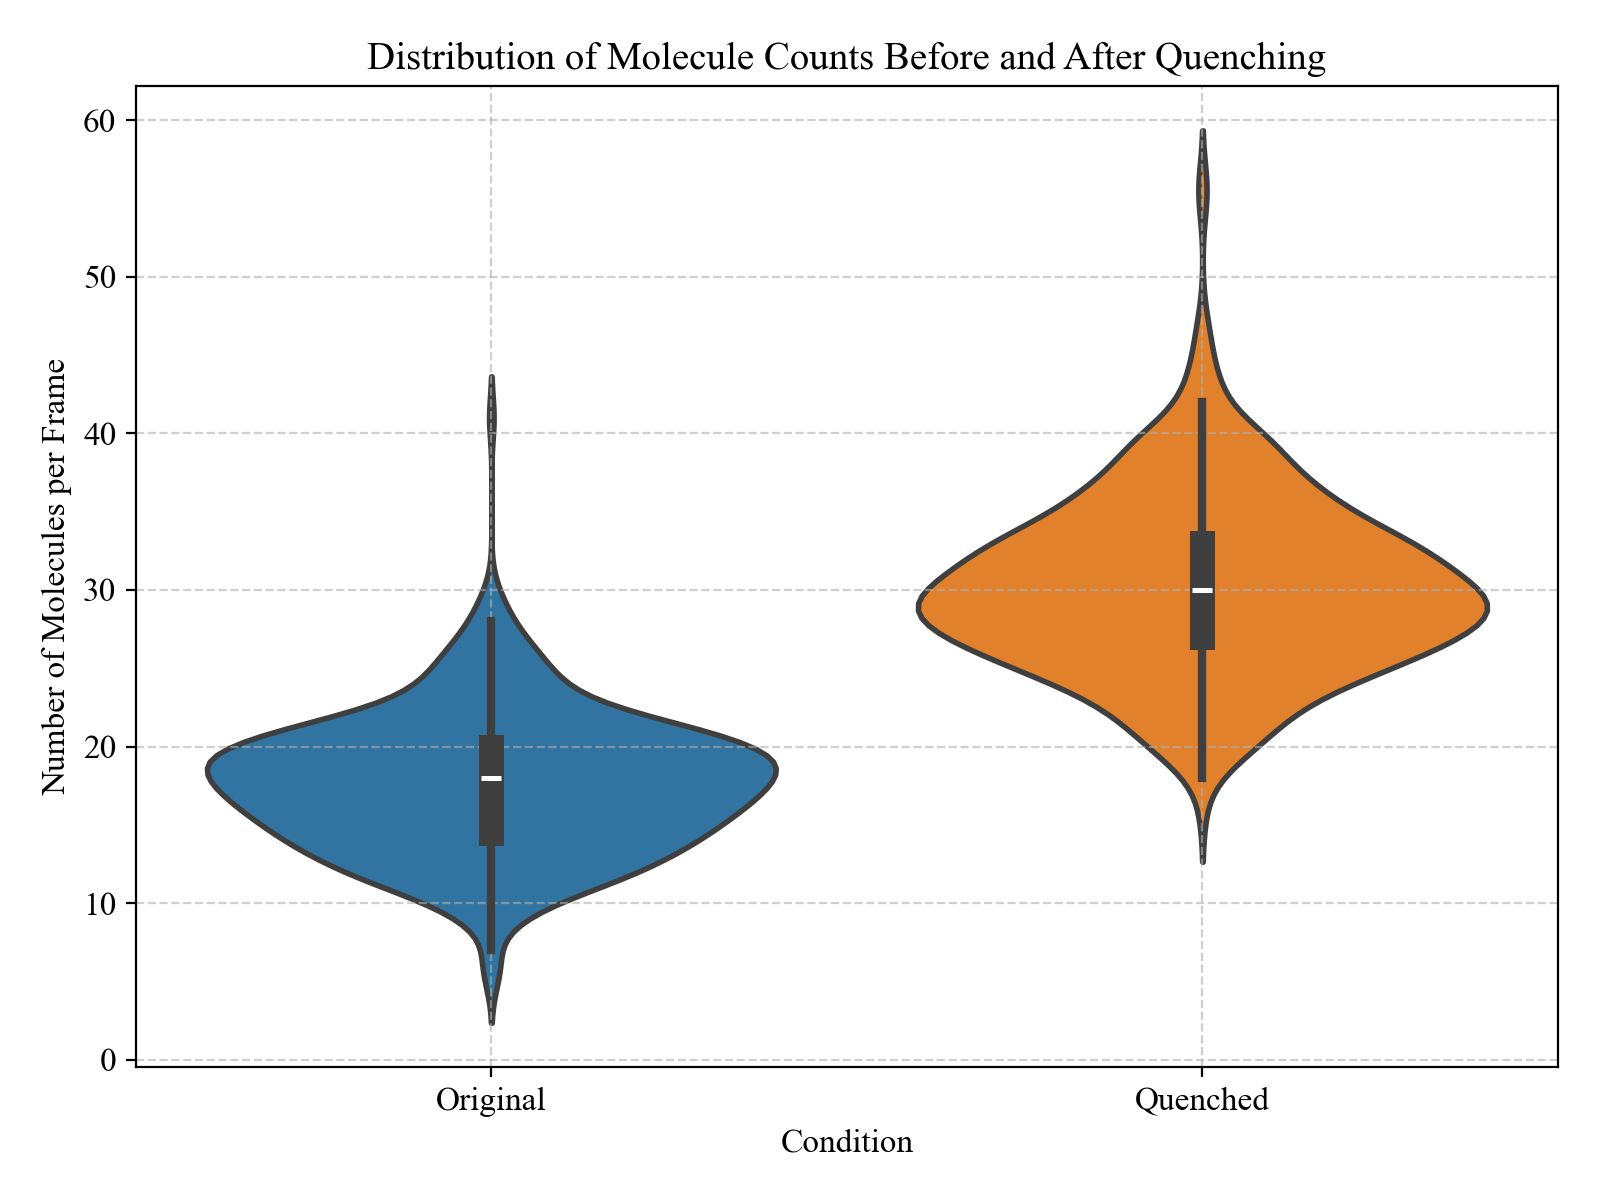
\includegraphics[width=1\linewidth]{Images/early_earth/violinplot-mol_counts-before-after-quench.png}
    \caption[Violin plot: total named molecules found before and after quenching large early earth system]{Distribution of per-frame counts of named molecules found before and after quenching 415 selected frames from the 22.8M atom system from 2500 K to 300 K.}
    \label{fig:ee_quench_violinplot}
\end{figure}

\section{Exploring new molecular configurations}
\label{sec:exploring_new_mol_configs}
As mentioned in \ref{subsec:drawback_config_sampling},
\hypertarget{configurational_sampling}{configuration sampling}
is difficult in the active learning via query by committee used in generating ANI datasets, and as a result new molecular configurations have been sampled from enumeration datasets and other curated chemical datasets.
The ANI-1xnr \cite{ani-1xnr} approach to generating training set data via nanoreactors and \authorRemark{other approaches taken in 1xnr paper serves as an inspiration for sampling new configurations from a massive batch of reaction data.}


\section{Interpretation of results}
\label{sec:hero_run_interpretation}

Initial search (detailed in ANI-1xnr and LAMMPS-ANI papers) in Sections \ref{sec:ani-1xnr} and \ref{sec:miller_experiment}.
Our initial search was for 357 molecules: the 20 proteinogenic amino acids (AAs), all possible dipeptides of those 20 AAs, ... \authorRemark{finish this list}.

From the initial search, using this limited list of biomolecules of interest, we counted nearly 6 million appearances of named biomolecules throughout the simulation.

\begin{table}[hb]
    \centering
    \begin{tabularx}{3in}{Xr}
        \hline
        Molecule name & Molecules identified \\
        \hline
        Glycine & 5,297,484 \\
        Alanine & 445,342 \\
        Serine & 2,183 \\
        Asparagine & 971 \\
        Valine & 591 \\
        Aspartic Acid & 439 \\
        Uracil & 414 \\
        Cytosine & 227 \\
        Threonine & 202 \\
        Caprylic acid & 137 \\
        Leucine & 46 \\
        Glutamine & 42 \\
        Glutamic Acid & 37 \\
        Isoleucine & 30 \\
        GlycylGlycine & 14 \\
        Lysine & 10 \\
        Thymine & 9 \\
        \hline
    \end{tabularx}
    \caption[Initial Early Earth molfind search]{The molecules identified in the initial analysis of the Hero Run data.}
    \label{tab:inital_molfind_counts}
\end{table}




Expanding the search:
Concomitant formation of protocells and prebiotic compounds under a plausible early Earth atmosphere: \cite{prebiotic_compounds_EE_atmosphere}\\
Abundant ammonia and nitrogen-rich soluble organic matter in samples from asteroid: \cite{astroid_sample}\\


